\documentclass[aspectratio=169]{beamer}
\usepackage[english]{babel}
\usepackage{amsthm}
\usepackage{mathtools}
\usepackage{physics}
\usepackage{calligra}
\usepackage{csquotes}
\usepackage{tensor}
\usepackage[thicklines]{cancel}
\usepackage{tcolorbox}
\usepackage{pstricks}
%\usepackage[backend=biblatex, bibstyle=nature, sorting=nty, citestyle=numeric-comp]{biblatex} %Custom bibliography
%    \addbibresource{bib.bib} %Load references


\DeclareMathAlphabet{\mathcalligra}{T1}{calligra}{m}{n}
\DeclareFontShape{T1}{calligra}{m}{n}{<->s*[2.2]callig15}{}
\newcommand{\scriptr}{\mathcalligra{r}\,}
\newcommand{\boldscriptr}{\pmb{\mathcalligra{r}}\,}
\def\rc{\scriptr}
\def\brc{\boldscriptr}
\def\hrc{\hat\brc}
\newcommand{\ie}{\emph{i.e.}} %id est
\newcommand{\eg}{\emph{e.g.}} %exempli gratia
\newcommand{\rtd}[1]{\ensuremath{\left\lfloor #1 \right\rfloor}}
\newcommand{\dirac}[1]{\ensuremath{\delta \left( #1 \right)}}
\newcommand{\diract}[1]{\ensuremath{\delta^3 \left( #1 \right)}}
\newcommand{\e}{\ensuremath{\epsilon_0}}
\newcommand{\m}{\ensuremath{\mu_0}}
\newcommand{\V}{\ensuremath{\mathcal{V}}}
\newcommand{\prnt}[1]{\ensuremath{\left(#1\right)}} %parentheses
\newcommand{\colch}[1]{\ensuremath{\left[#1\right]}} %square brackets
\newcommand{\chave}[1]{\ensuremath{\left\{#1\right\}}}  %curly brackets

\useoutertheme{infolines}
\useinnertheme{rectangles}
\usefonttheme{professionalfonts}


%\definecolor{orange}{HTML}{f28165}
%\definecolor{gray}{HTML}{303030}
%\definecolor{yellow}{HTML}{f0be52}
%\definecolor{lightorange}{HTML}{f19e58}

\definecolor{orange}{HTML}{5555ff}
\definecolor{gray}{HTML}{303030}
\definecolor{yellow}{HTML}{111152}
\definecolor{lightorange}{HTML}{2222dd}

\renewcommand{\CancelColor}{\color{orange}}

\makeatletter
\newcommand{\mybox}[1]{%
  \setbox0=\hbox{#1}%
  \setlength{\@tempdima}{\dimexpr\wd0+13pt}%
  \begin{tcolorbox}[colback=orange,colframe=orange,boxrule=0.5pt,arc=4pt,
      left=6pt,right=6pt,top=6pt,bottom=6pt,boxsep=0pt,width=\@tempdima]
    \textcolor{white}{#1}
  \end{tcolorbox}
}
\makeatother

\usecolortheme[named=orange]{structure}
\usecolortheme{sidebartab}
\usecolortheme{orchid}
\usecolortheme{whale}
\setbeamercolor{alerted text}{fg=yellow}
\setbeamercolor{block title alerted}{bg=alerted text.fg!90!black}
\setbeamercolor{block title example}{bg=lightorange!60!black}
\setbeamercolor{background canvas}{bg=gray}
\setbeamercolor{normal text}{bg=gray,fg=white}

\setbeamertemplate{footline}
        {
      \leavevmode%
      \hbox{%
      \begin{beamercolorbox}[wd=.333333\paperwidth,ht=2.25ex,dp=1ex,center]{author in head/foot}%
        \usebeamerfont{author in head/foot}\insertshortauthor~~(\insertshortinstitute)
      \end{beamercolorbox}%
      \begin{beamercolorbox}[wd=.333333\paperwidth,ht=2.25ex,dp=1ex,center]{title in head/foot}%
        \usebeamerfont{title in head/foot}\insertshorttitle
      \end{beamercolorbox}%
      \begin{beamercolorbox}[wd=.333333\paperwidth,ht=2.25ex,dp=1ex,center]{date in head/foot}%
        \usebeamerfont{date in head/foot}\insertshortdate{}%\hspace*{2em}

    %#turning the next line into a comment, erases the frame numbers
        %\insertframenumber{} / \inserttotalframenumber\hspace*{2ex} 

      \end{beamercolorbox}}%
      \vskip0pt%
    }


\setbeamertemplate{blocks}[rectangle]
\setbeamercovered{dynamic}

\setbeamertemplate{section page}
{
	\begin{centering}
		\begin{beamercolorbox}[sep=27pt,center]{part title}
			\usebeamerfont{section title}\insertsection\par
			\usebeamerfont{subsection title}\insertsubsection\par
		\end{beamercolorbox}
	\end{centering}
}

%\setbeamertemplate{subsection page}
%{
%	\begin{centering}
%		\begin{beamercolorbox}[sep=12pt,center]{part title}
%			\usebeamerfont{subsection title}\insertsubsection\par
%		\end{beamercolorbox}
%	\end{centering}
%}

\newcommand{\hlight}[1]{\colorbox{violet!50}{#1}}
\newcommand{\hlighta}[1]{\colorbox{red!50}{#1}}
\title{Evaluation of gate designs} %->->->->-> Check hyperref title <-<-<-<-<-
\subtitle{For trapped ion quantum computers}
\author[L. Pal\' anki]{Lajos Pal\' anki}
\institute[ICL]{
    Department of Physics%
    \\%
    Imperial College London%
} %You can change the Institution if you are from somewhere else
\date{March 25, 2022}
%\logo{\includegraphics[width= 0.2\textwidth]{images/a-logo.png}}
\usepackage[style=ieee,backend=bibtex]{biblatex}
\usepackage[percent]{overpic}
\addbibresource{sources.bib}
\DeclareFieldFormat{labelnumberwidth}{}
\setlength{\biblabelsep}{0pt} 
\beamertemplatenavigationsymbolsempty
\begin{document}
    
    \frame{\titlepage}
    
%    \begin{frame}{Summary}
%        \tableofcontents
%    \end{frame}
    
    %\input{chapters/a-silly-idea.tex} %You can put the frames directly into the presentation, but using the input command and writing them in separate .tex files might be more organized
    
    %\input{chapters/playing-around.tex}
    
    %\input{chapters/fourier-playground.tex}
    
    \section{Background}
    %\frame{\sectionpage}
	\begin{frame}{Energy structure}
		\begin{figure}
			\centering
			\only<1>{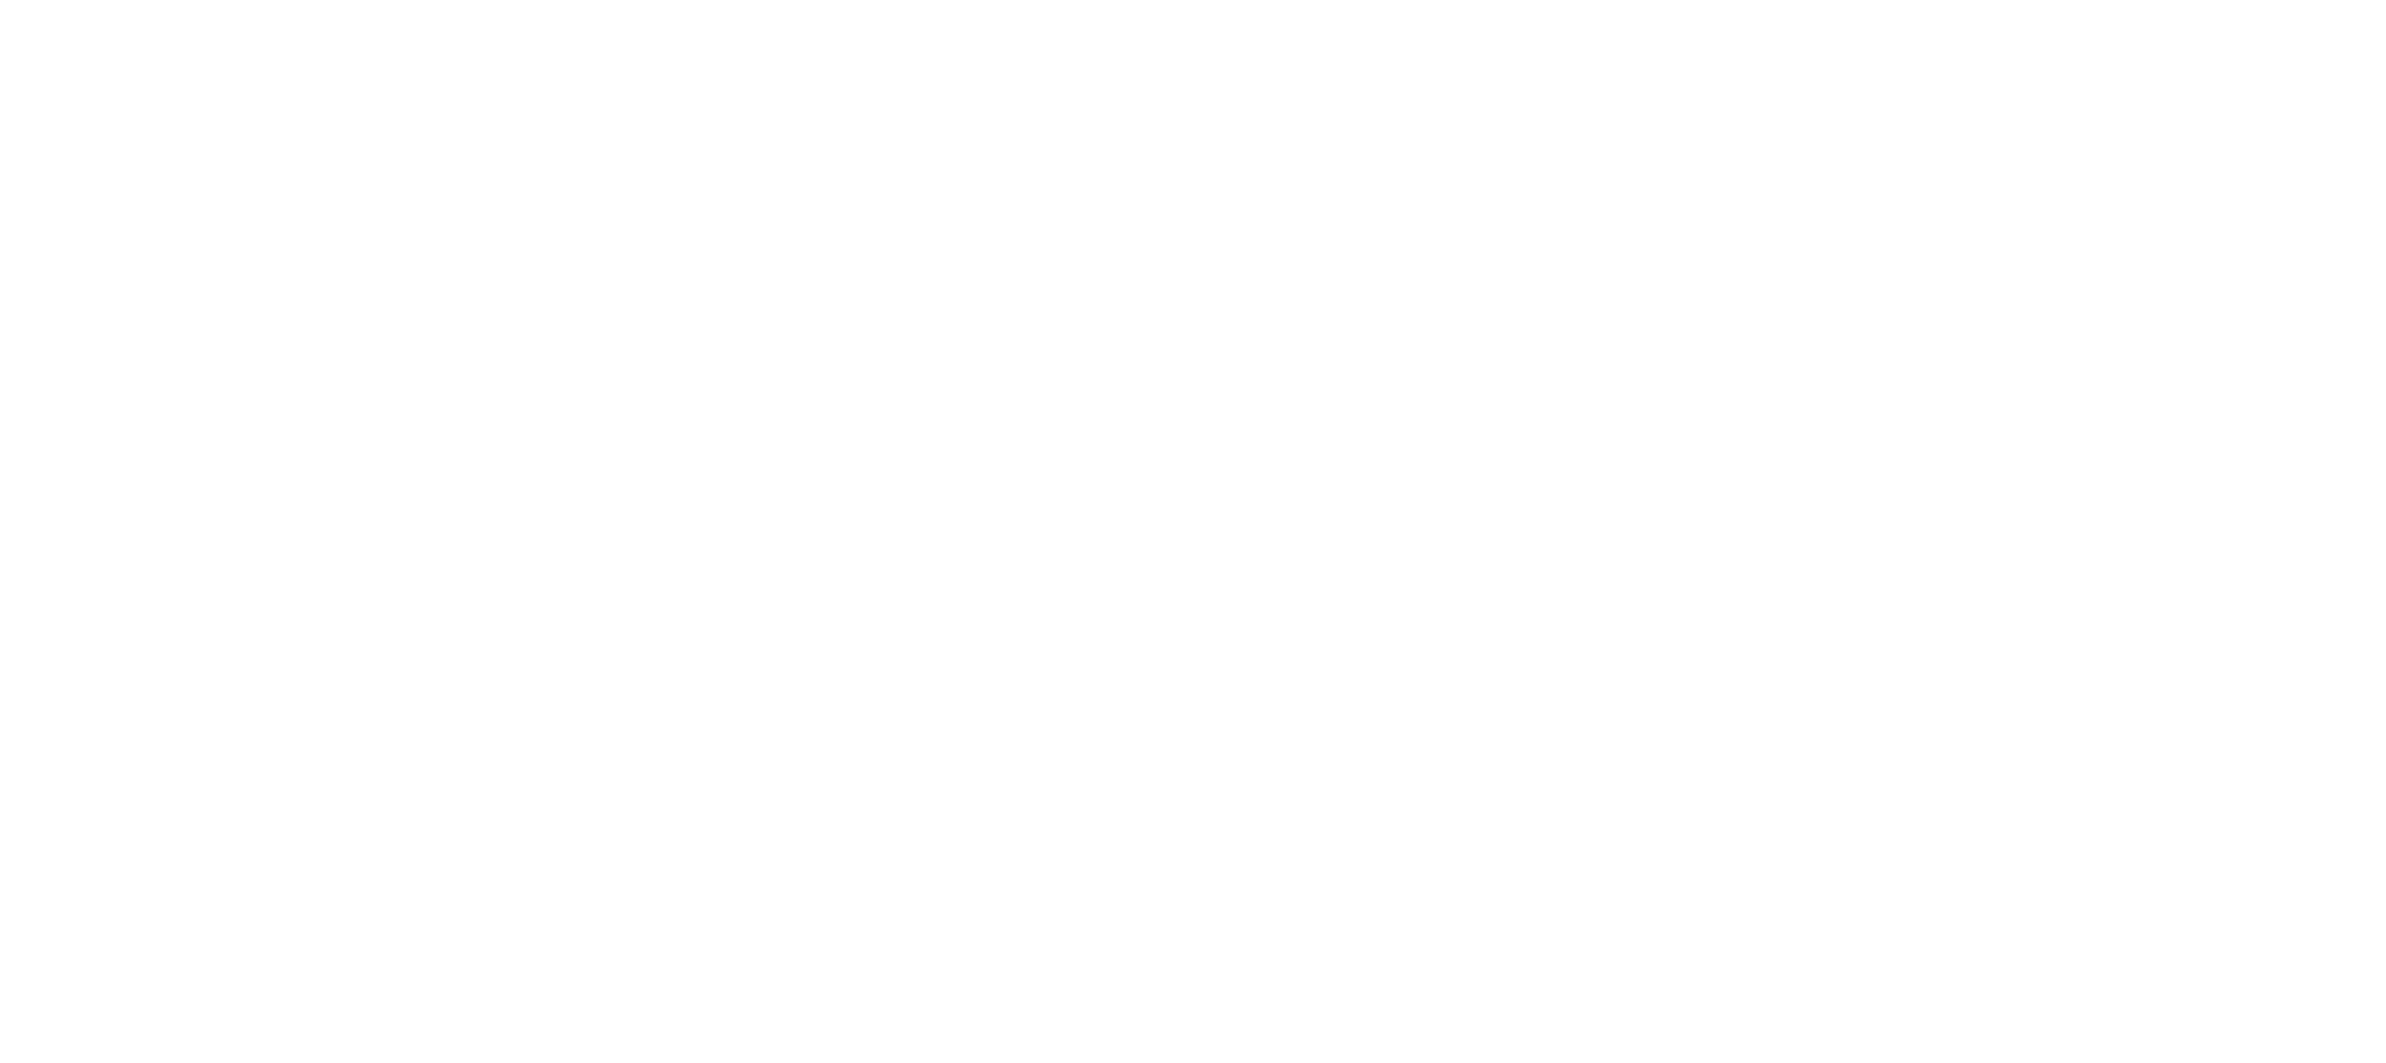
\includegraphics[width=0.75\linewidth]{1ion_Elevels.pdf}}
			\only<2-3>{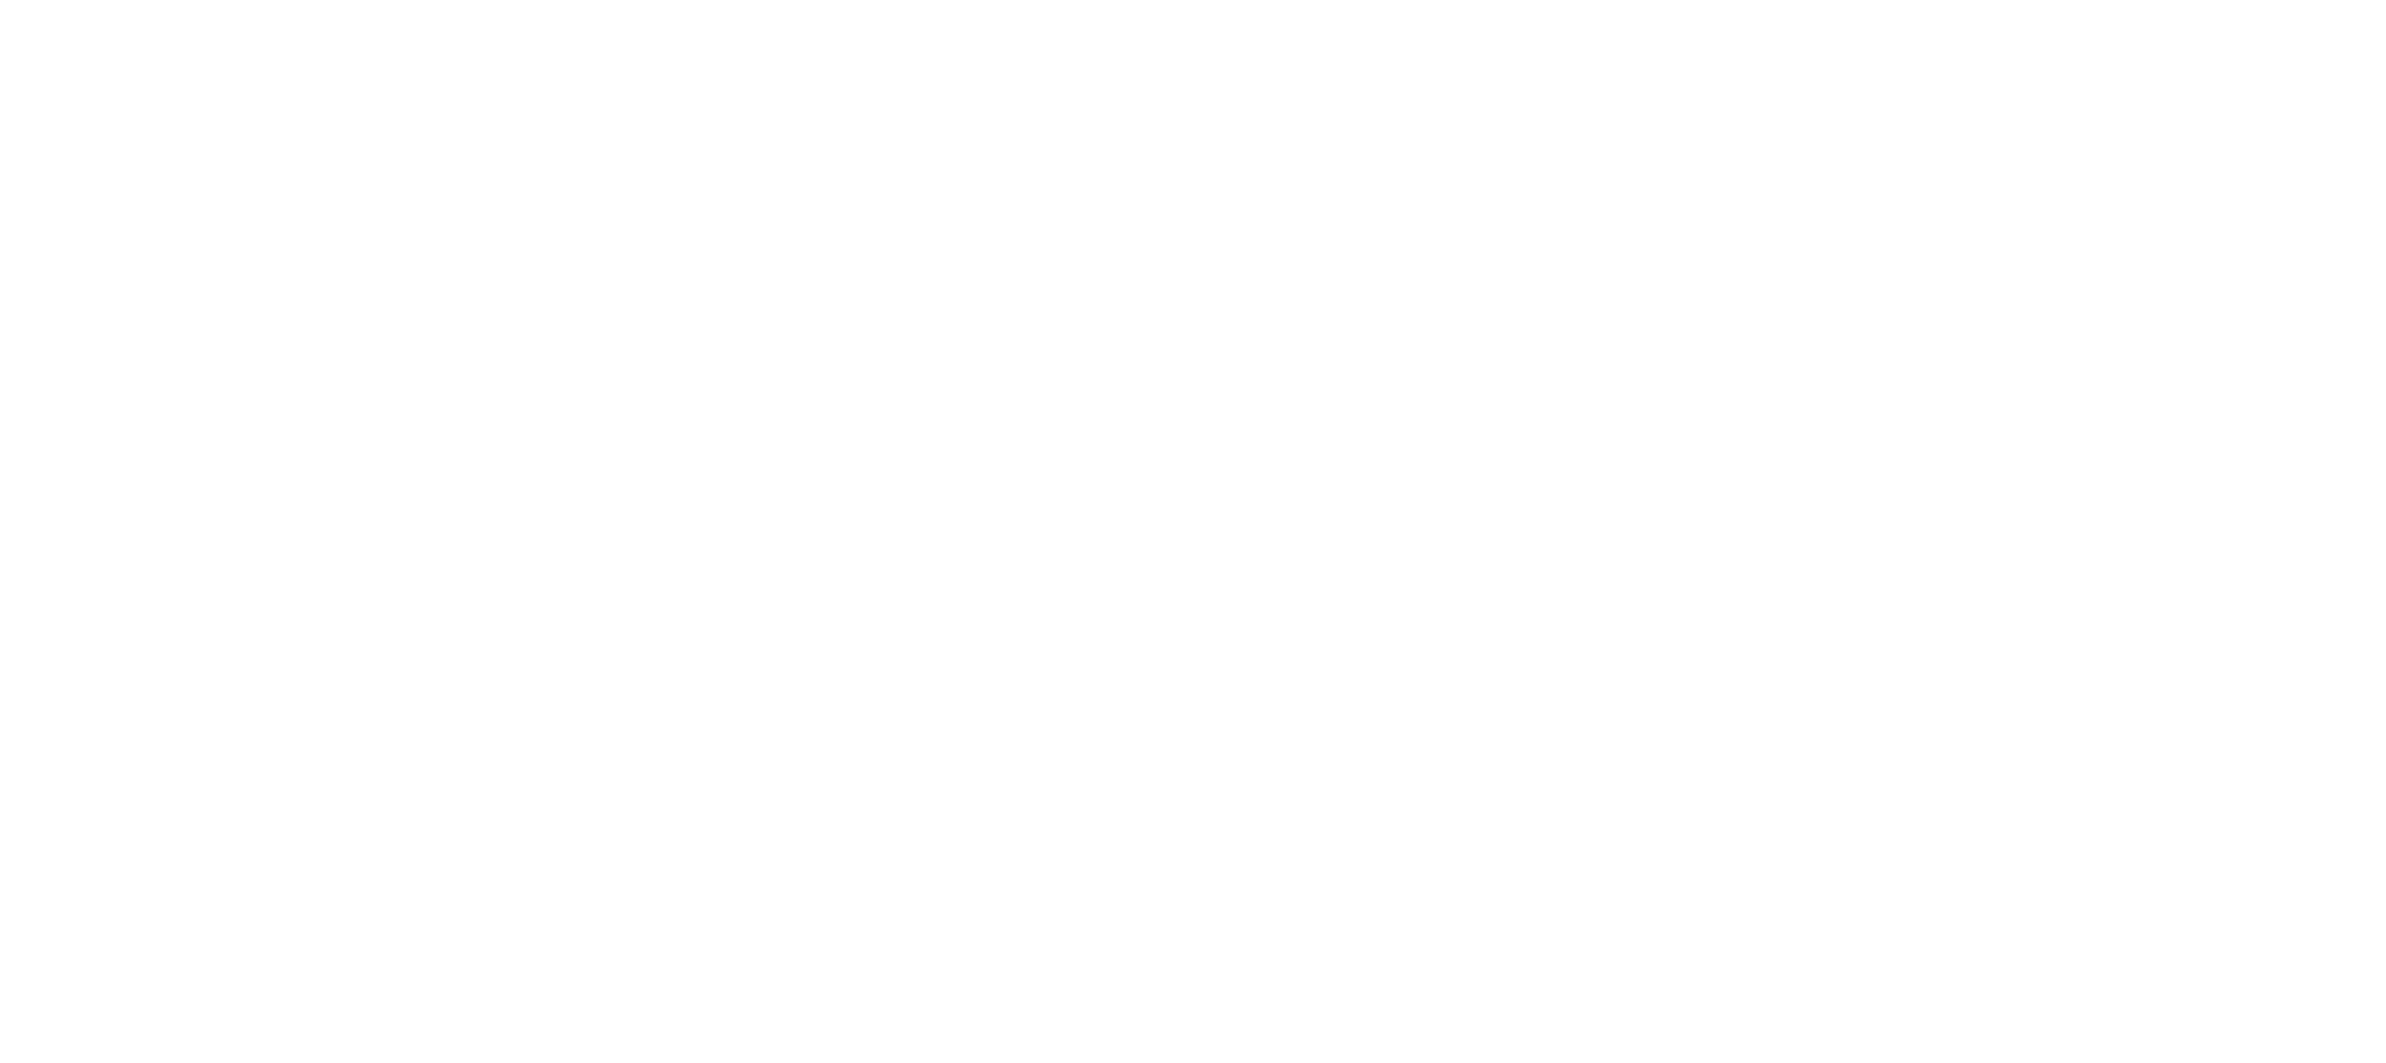
\includegraphics[width=0.75\linewidth]{2ion_Elevels.pdf}}
			\only<3>{\vspace{0.57em}}
			\[\hat{H}=-\frac{\hbar\omega_0}{2}\only<1>{\hat{\sigma}_z}\only<2>{\sum_i^n\hat{\sigma}_z^{(i)}}\only<3>{\hat{S}_z}+ \hbar\nu \left(\hat{a}^\dagger\hat{a} + \frac{1}{2}\right)\]
		\end{figure}
	\end{frame}
    \begin{frame}{Driving the system}
    	\begin{align*}
    		\onslide<1->{\hat{H}&=-\frac{\hbar\omega_0}{2}\hat{S}_z+ \hbar\nu \left(\hat{a}^\dagger\hat{a} + \frac{1}{2}\right) + \sum_{i}\frac{\Omega_i}{2}\hat{S}_+e^{-i\left(\mathbf{kz}-\omega_i t\right)} + h.c.}\\
    		\onslide<2->{\hat{H}&=-\frac{\hbar\omega_0}{2}\hat{S}_z+ \hbar\nu \left(\hat{a}^\dagger\hat{a} + \frac{1}{2}\right) + \sum_{i}\frac{\Omega_i}{2}\hat{S}_+e^{-i\left(\eta\left(\hat{a}+\hat{a}^\dagger\right) -\omega_i t\right)} + h.c.}\\
    		\onslide<3->{\hat{H}_I&=\sum_{i}\frac{\Omega_i}{2}\hat{S}_+e^{-i\left(\eta\left(\hat{\tilde{a}}+\hat{\tilde{a}}^\dagger\right) -\Delta_i t\right)} + h.c.}
    	\end{align*}
    	\[\onslide<2->{\eta = \mathbf{kz_0}}\onslide<3->{\hspace{5em}\hat{\tilde{a}}=\hat{a}e^{-i\nu t}\hspace{5em}\hat{\tilde{a}}^\dagger =\hat{a}^\dagger e^{i\nu t}}\]
    \end{frame}

	\section{Driving schemes}
	\begin{frame}{M\o lmer-S\o rensen gate}
		\centering
		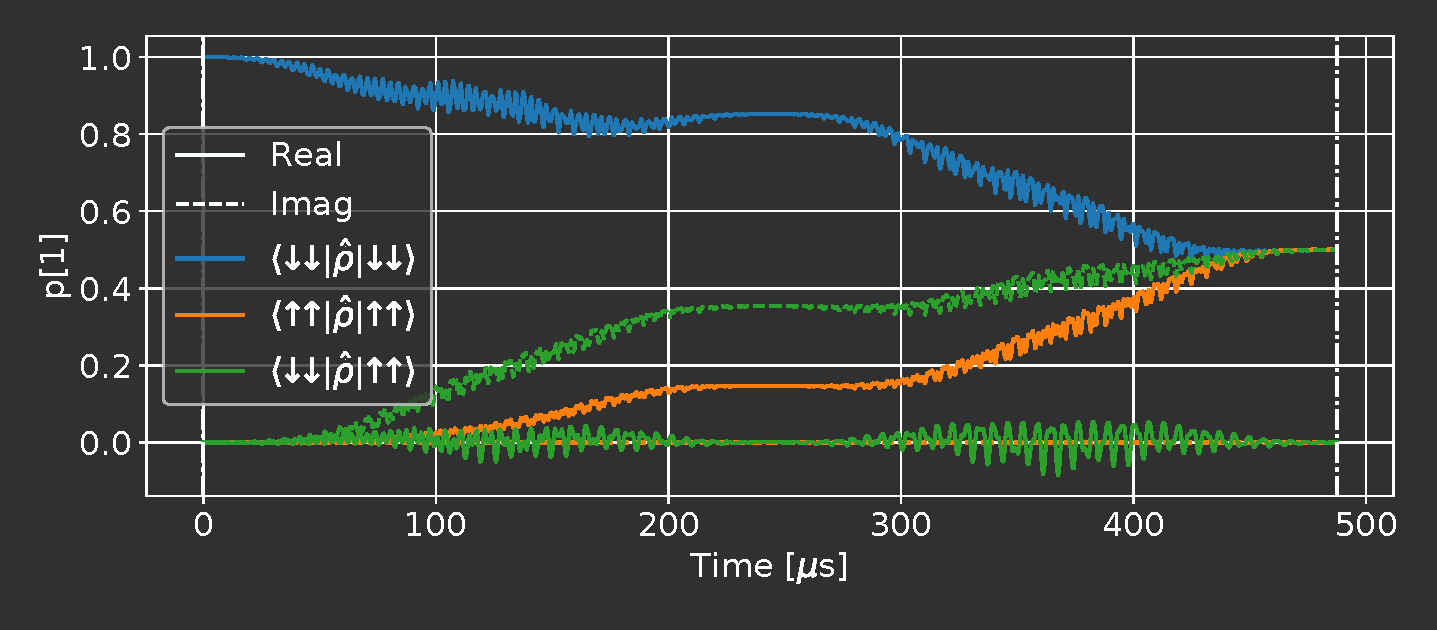
\includegraphics[height=12.5em]{test.pdf}
		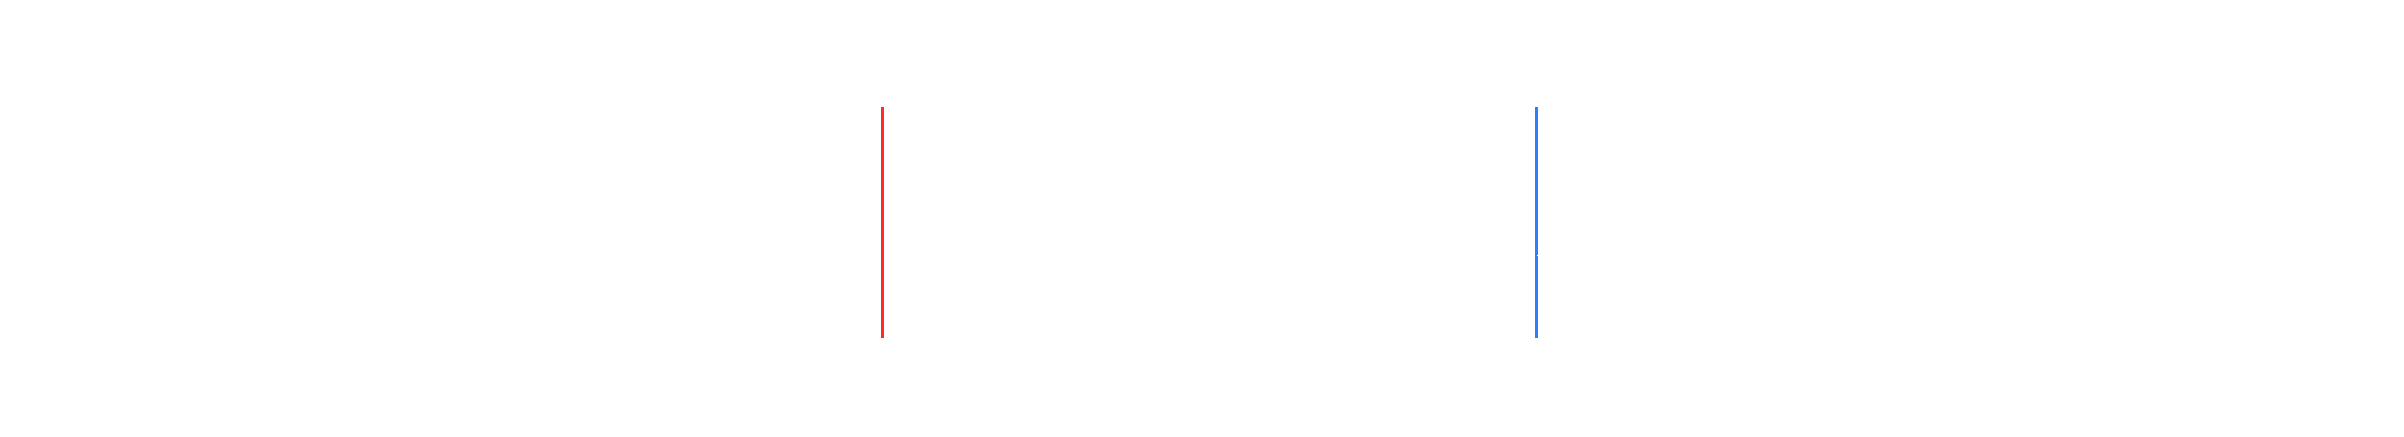
\includegraphics[width=0.75\linewidth]{MS-gate.pdf}
	\end{frame}
	\begin{frame}{Strong coupling gate}
		\centering
		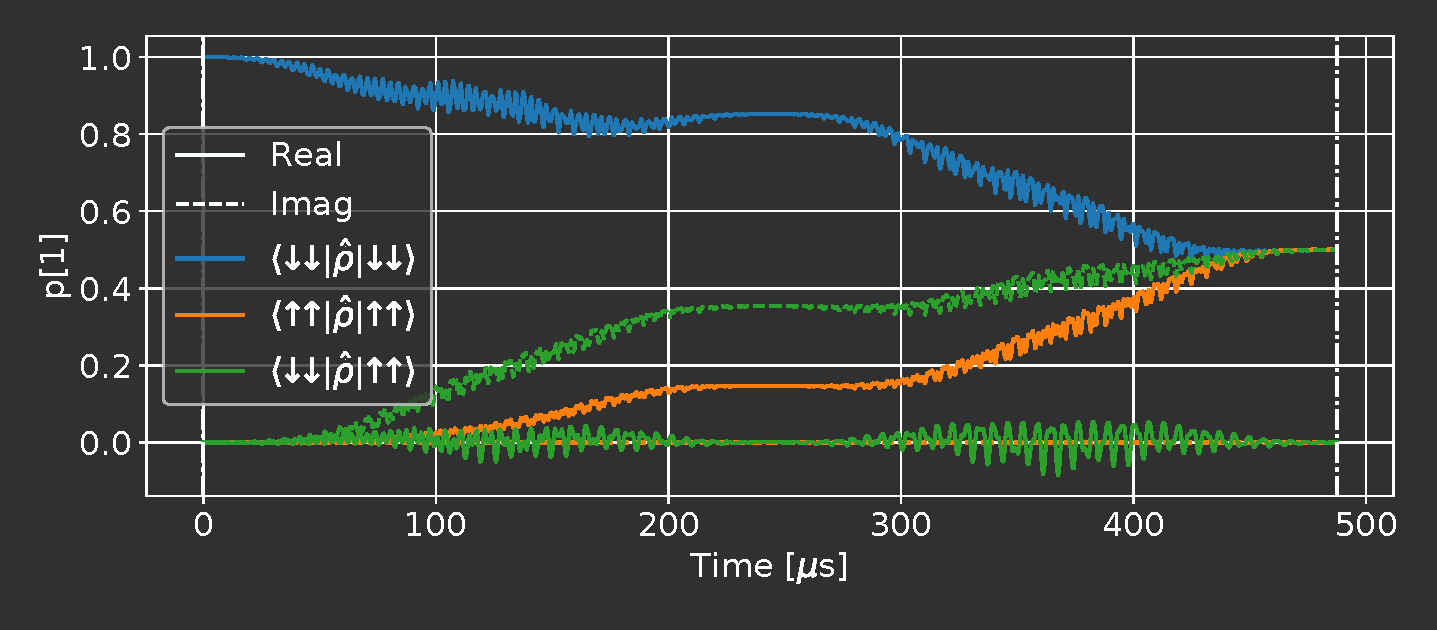
\includegraphics[height=12.5em]{test.pdf}
		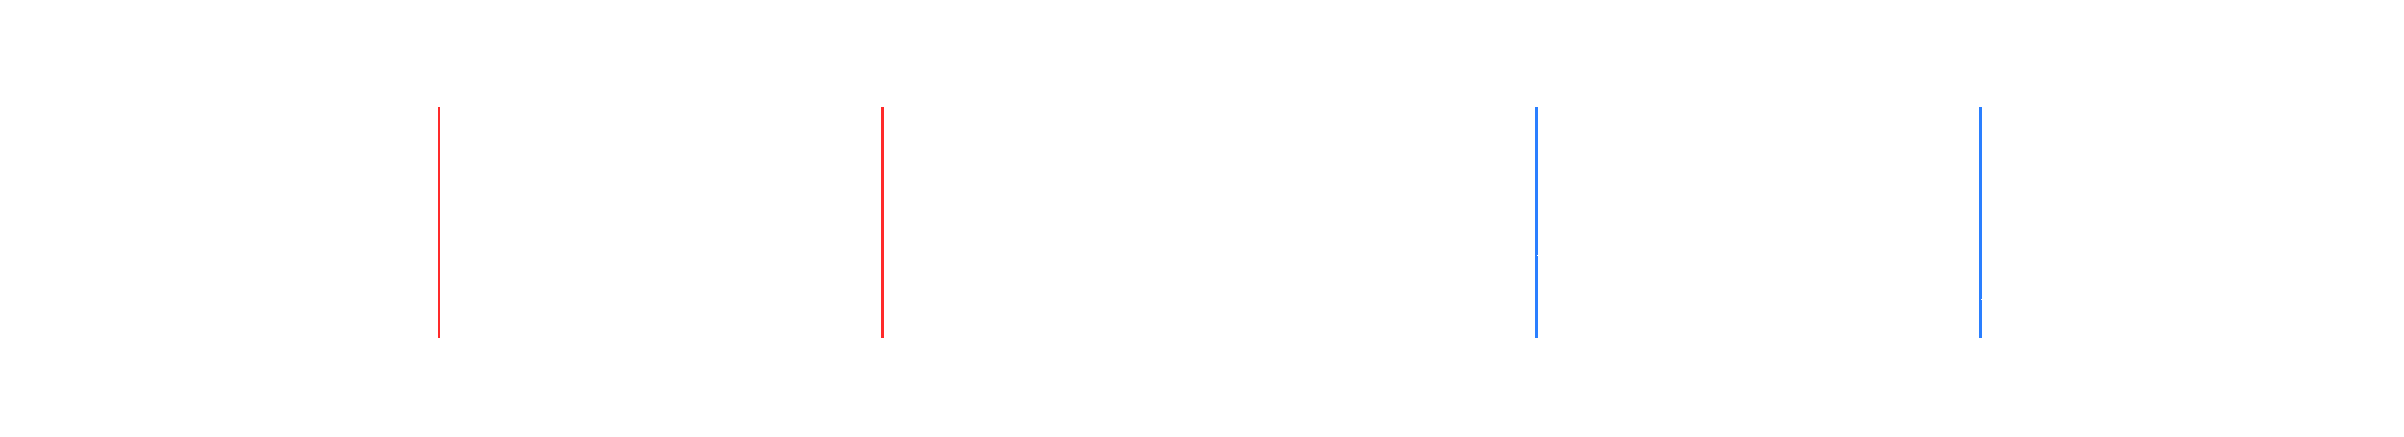
\includegraphics[width=0.75\linewidth]{SC2-gate.pdf}
	\end{frame}
	\begin{frame}{Cardioid gate}
		\centering
		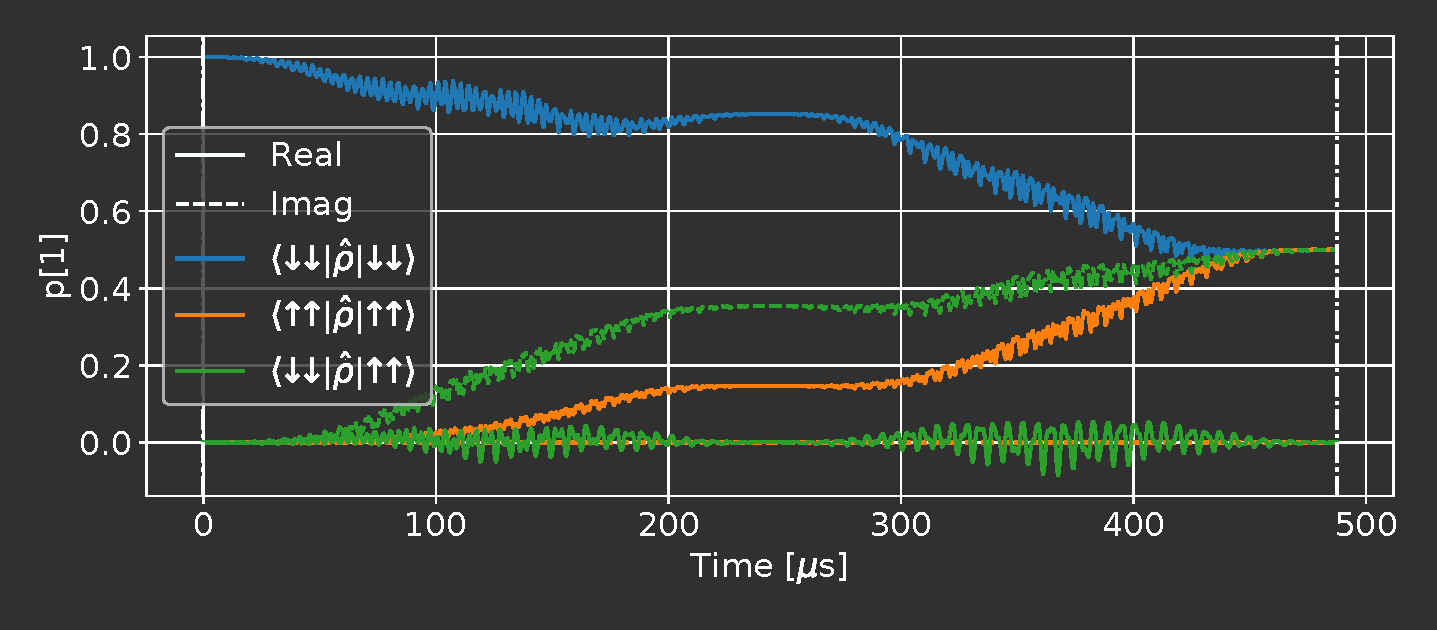
\includegraphics[height=12.5em]{test.pdf}
		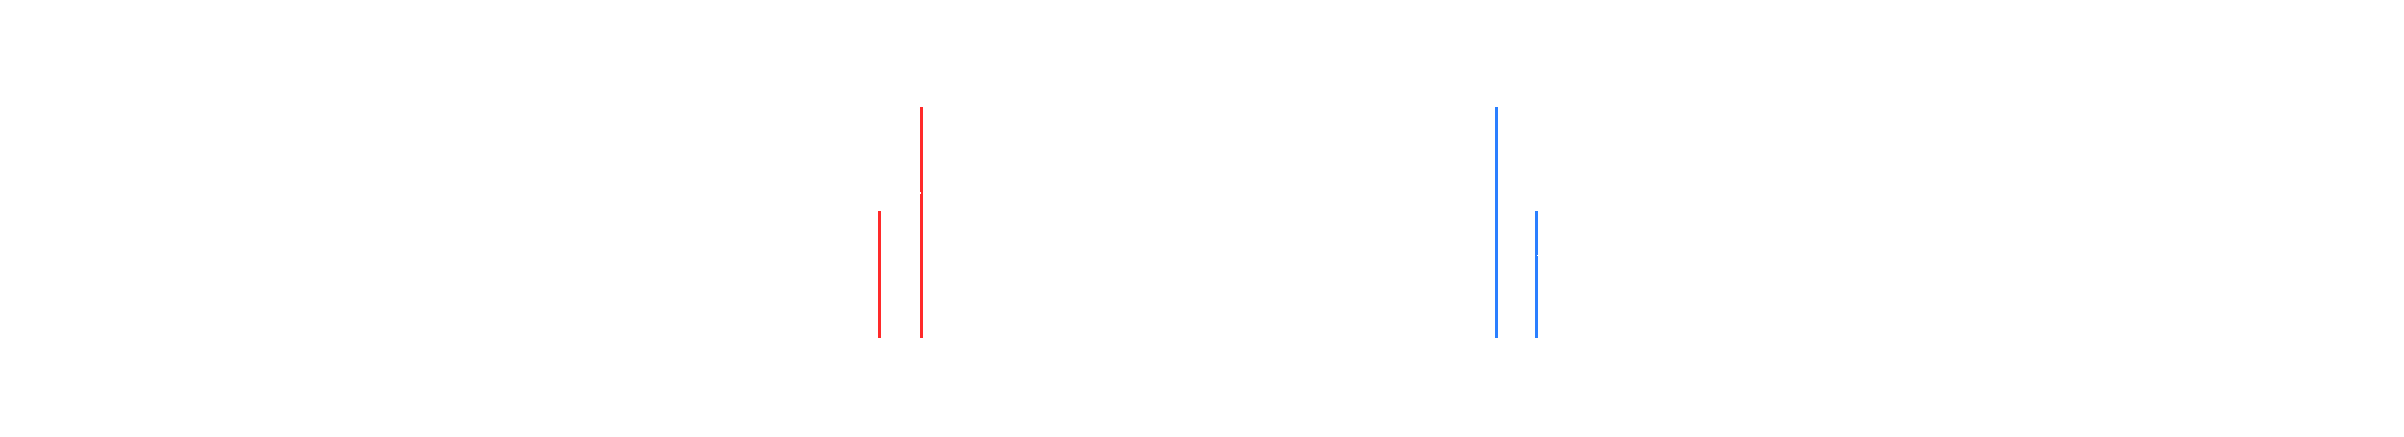
\includegraphics[width=0.75\linewidth]{Cardioid-gate.pdf}
	\end{frame}
	\begin{frame}{Compound gate}
		\centering
		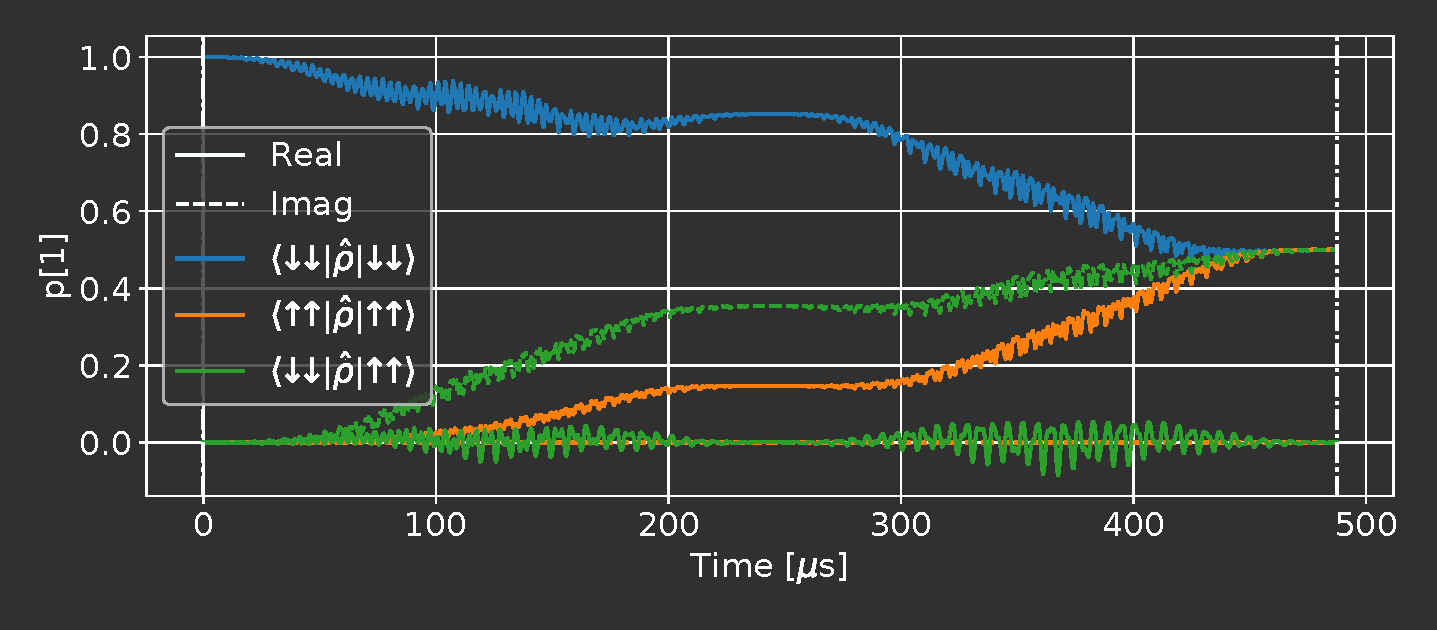
\includegraphics[height=12.5em]{test.pdf}
		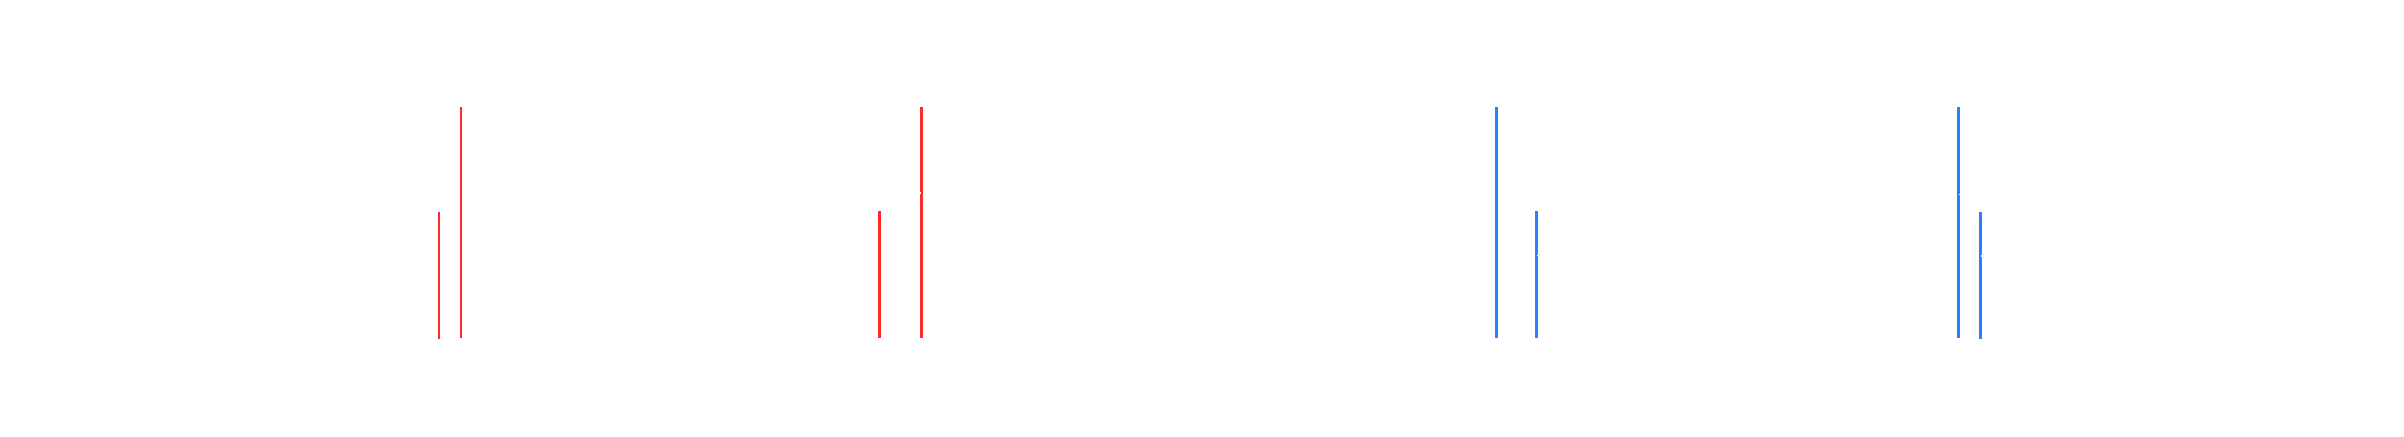
\includegraphics[width=0.75\linewidth]{Compound-gate.pdf}
	\end{frame}

%    \section*{Acknowledgments} %You can remove this if you do not want to use it
%        \begin{frame}{Acknowledgments}
%            The author is extremely thankful to Prof. Antônio F. R. T. Piza for the short, yet wonderful, conversations about this seminar.
%        \end{frame}

%    \section{}
%    \begin{frame}{}
%        \centering
%            \Huge\bfseries
%        \textcolor{orange}{The End}
%    \end{frame}
\end{document}
